\chapter{Fejlesztői dokumentáció}
\label{ch:impl}

Ebben a fejezetben az általam létrehozott szoftver működését mutatom be.
A szoftver felépítését, a felhasznált tervezési mintákat és
a fontosabb algoritmusok működését is bemutatom.
A szoftver forráskódja a jövőben változhat,
a frissített API dokumentáció ezért a személyes oldalamon is elérhető \cite{apidoc}.

\section{Csomagok}

A szoftver forráskódja több csomagban és modulban található.
Minden csomag a szoftver egy jól elkülöníthető rétegét valósítja meg,
például az alkalmazási réteget vagy az átalakításokért felelő réteget.

A forráskód öt csomagba van szerveze, ezek az alábbi táblázatban láthatóak.

\begin{table}[H]
	\centering
	\begin{tabular}{ | m{0.25\textwidth} | m{0.65\textwidth} | }
		\hline
		\textbf{Csomag} & \textbf{Rövid leírás} \\
		\hline \hline
		\emph{transformations} & átalakítások forráskódja és API az átalakításokhoz \\
		\hline
		\emph{client} & adatbázis kliens \\
		\hline
		\emph{model} & adatok modellezése és mentése \\
		\hline
		\emph{app} & GUI alkalmazás csomagja \\
		\hline
		\emph{tests} & egység és egyéb tesztek \\
		\hline
	\end{tabular}
	\caption{A szoftver fő csomagjai}
	\label{tab:packages}
\end{table}

Az szoftver "futtatható" fájljai és fontosabb függvényei
a csomagokon kívül, külön modulokban helyezkednek el.
A modulokról a \ref{sec:modules}. szekcióban olvashatunk.

\section{A \emph{transformations} csomag}

Ebben a szekcióban ismertetem a \emph{transformations} csomagot.
Bemutatom az átalakításokhoz használt \emph{ast} modult és
az általam implementált átalakítások működését is részletezem.

\subsection{Az \emph{ast} modul}

Az átalakításokat a Python \emph{ast} moduljával valósítottam meg.
Az \emph{ast} modul a Python standard könyvárában alapból megtalálható, 
célja az AST létrehozása a Python absztrakt-nyelvtanának alapján.

A Python absztrakt-nyelvtana a nyelv szintaxisát leíró környezetfüggetlen nyelvtan,
definícióját az \emph{ast} modul dokumentációjának \cite{pythonAST} elején találjuk.

Az absztrakt-nyelvtan definíciójában az AST csúcsainak (node-jainak) típusát az
\emph{ast.AST}-ből származó osztályok határozzák meg,
ezekről szintén a dokumentáció elején, a \emph{Node classes} cím alatt olvashatunk.
Egy AST-re tehát általánosan az \emph{ast.AST} osztállyal hivatkozhatunk.

Egy Python forráskód AST-jét az \emph{ast.parse} függvénnyel hozhatjuk létre.
Az \emph{ast.parse} ekvivalens a Python beépített
\emph{compile} függvényének \texttt{ast.PyCF\_ONLY\_AST} compiler flaggel való
meghívásával.

Fontos, hogy AST-t csak olyan forráskódból tudunk létrehozni, amiben nincs
szintaxis hiba.
A szintaxis hibákat az \emph{ast.parse} a \emph{SyntaxError} exceptionnel jelzi.

Az \emph{ast} modulban AST-k bejárására és átalakítására alkalmas
segédfüggvények és segédosztályok is találhatóak.
Az általam megvalósított átalakításokban
az AST bejárását a \emph{NodeVisitor} osztállyal,
az AST átalakítását pedig a \emph{NodeTransformer} osztállyal
végzem.

Az átalakított AST-ből a kód generálására az \emph{ast.unparse} függvényt használom.
Fontos megjegyezni, hogy az \emph{unparse} függvénnyel generált kód nem garantáltan
helyes szemantikus szinten.

Az általam implementált átalakítások az egyszerűség kedvéért feltételezik a bemeneti
kódok szemantikus helyességét.


\subsubsection{A \emph{NodeVisitor} osztály}

Az AST-ket a \emph{NodeVisitor} osztályból származtatott osztályokkal járhatjuk be.

A \emph{NodeVisitor}-ból származtatott osztályokkal olyan, AST-vel kapcsolatos,
lekérdezéseket is reprezentálhatunk, amelyek elvégzéséhez az AST bejárása szükséges.

Például egy AST-ben, az adott id-vel rendelkező, \emph{Name} node-ok listáját
a \ref{src:NameVisitor}. forráskódon látható \emph{NameVisitor} osztály
\emph{get\_names} metódusával kaphatjuk meg.

\lstset{caption={A \emph{NameVisitor} osztály kódja}, label=src:NameVisitor}
\begin{lstlisting}[language={Python}]
	class NameVisitor(NodeVisitor):
		
		def get_names(self, root: AST, id: str) -> list:
			self._id = id
			self._names = []
			self.visit(root)
			return self._names
		
		def visit_Name(self, node: ast.Name):
			if self._id == node.id:
				self._names.append(node)
\end{lstlisting}

A \emph{get\_names} metódus paraméterei az AST (\emph{root}) és a keresett id (\emph{id}).
Először a metódus inicializálja az \emph{\_id} és \emph{\_names} példány szintű változókat,
majd elindítja a bejárást a \emph{root}-ra.
Bejárás után visszaadja a \emph{\_names}-ben összegyűjtött \emph{Name} node-ok listáját.

A bejárást a \emph{NodeVisitor} osztályból örökölt \emph{visit} metódus meghívásával
lehet elindítani egy AST-re. Ez a bejárás \textbf{mélységi bejárás}.

Bejárás közben a \emph{Name} node-okat a \emph{NodeVisitor} osztály \emph{visit\_Name}
metdódusának felülírásával látogatjuk meg.
A meglátogatott \emph{Name} node-ot akkor adjuk a listához,
ha az id-je egyezik az \emph{\_id}-vel.

Ehhez a példához hasonlóan a \emph{NodeVisitor}-ban az összes node típushoz
létezik \emph{visit\_<node-class>} visitor metódus amit felülírhatunk.

Fontos megjegyezni, hogy amikor felülírjuk a visitor metódust olyan node-típusoknál
amik tartalmazhatnak magukkal megegyező típusú node-ot (például \emph{For} node),
akkor az összes node meglátogatásához szükséges a \emph{generic\_visit} hívása
a felülírt metódusban, különben a rekurzió megáll.

\emph{NodeVisitor}-ból származtatott osztállyal akkor érdemes bejárást végezni,
ha mélységi bejárásra van szükségünk.

Amikor egy \emph{NodeVisitor}-ból származtatott osztályban a bejárás rekurzív hívása történik,
minden gyerekre a gyerek típusához tartozó visitor metódus kerül meghívásra, ha az létezik.
Tehát, ha a gyerek típusának visitor metódusát felülírtuk, akkor a gyereket azzal fogja meglátogatni.
Ha nem írtuk felül, akkor a \emph{NodeVisitor} osztály
\emph{generic\_visit} metódusa a node-okat mélységi sorrendben látogatja meg.
Ezért folytat a \emph{NodeVisitor} alapból mélységi bejárást.

A \emph{generic\_visit}-et is felülírhatjuk.
Erre a \ref{src:TypeVisitor}. forrráskódban láthatunk példát.

\lstset{caption={A \emph{TypeVisitor} osztály kódja}, label=src:TypeVisitor}
\begin{lstlisting}[language={Python}]
	class TypeVisitor(NodeVisitor):
		
		def get_nodes(self, root: AST,
			node_matcher: Callable[[AST], bool]
		) -> list:
			self._node_matcher = node_matcher
			self._nodes = []
			self.visit(root)
			return self._nodes
		
		def generic_visit(self, node: AST):
			super().generic_visit(node)
			if self._node_matcher(node):
				self._nodes.append(node)
\end{lstlisting}


A \ref{src:TypeVisitor}. forráskódban definiált \emph{TypeVisitor} osztály
a \ref{src:NameVisitor}. forráskódban definiált \emph{NameVisitor} osztály
általánosítása.

A \emph{TypeVisitor} a bejárt AST azon a node-jait adja vissza,
amikre a paraméterül kapott \emph{node\_matcher}, $AST \rightarrow bool$ típusú,
függvény igaz értéket adott vissza.
Ez a függvény egy node valamilyen tulajdonságát határozza meg,
vagyis több típusú node-ra is működhet.
Ezért kell a \emph{generic\_visit}-et használni,
amivel az összes AST-ben található node-ot meglátogathatjuk.

\subsubsection{A \emph{NodeTransformer} osztály}

Az AST-k átalakítása a \emph{NodeTransformer} osztály segítségével valósítható meg.
Ez az osztály kimondottan erre a célra használandó.

A \emph{NodeVisitor}-hoz hasonlóan a \emph{NodeTransformer}-ből is származtatni
kell az osztályokat.
Mivel a \emph{NodeTransformer} maga is a \emph{NodeVisitor} osztályból származik,
a működése nagyon hasonló.

A bejárás szinte ugyanúgy működik mint a \emph{NodeVisitor}-ban.
Az AST-t itt is a \emph{generic\_visit} vagy \emph{visit\_<node-class>} metódusokkal
járhatjuk be.
A különbség az, hogy az éppen meglátogatott node-ot a
\emph{generic\_visit} vagy \emph{visit\_<node-class>}
metódusok visszatérési értékével lehet változtatni. 

Ha a bejárás közben a node-ot meglátogató függvény visszatérési értéke \texttt{None},
akkor a meglátogatott node törlődik az AST-ből.

Ha a node-ot meglátogató függvény visszatérési értéke nem \texttt{None},
hanem egy \emph{ast.AST} típusú node,
akkor a meglátogatott node a visszaadott node-ra változik az AST-ben
(ha a node-on nem akarunk változtatni akkor változatlanul visszaadjuk).

\subsection{Az átalakítások működése}

Egy átalakítás, működése (magas szinten) a következő lépésekből áll:

\begin{enumerate}
	\item AST létrehozása egy kódból
	\item AST bejárása és elemzése
	\item AST bejárása és átalakítása
	\item kód generálása az AST-ből
\end{enumerate}

Az átalakításokat végző algoritmusok a \emph{transformers}, \emph{transformers\_rename}
és \emph{visitors} modulokban találhatóak, ezek a modulok tartalmazzák az AST-t
elemző és változtató osztályokat is.

Az általam definiált átalakítások közül egyedül
a \emph{transformers\_rename} modulban található átnevezéses
átalakítások nem használnak szabályokat.
Minden más átalakítás szabályokra épül.

\subsection{Szabályok}

Egy szabály az AST egy node-ján vagyis részfáján alkalmazható.
Alkalmazásának két lépése van, amit két, AST-n értelmezett, függvény reprezentál:

\begin{enumerate}
	\item mintaillesztés az adott node-on:
	
	\(match(node: AST) -> Any | None \)
	
	\item eredmény generálása és visszaadása:
	
	\(change(node: AST) -> Any | None \)
\end{enumerate}

A két lépésnek megfelelő metódusokat a szabályok absztrakt típusát definiáló
\emph{transformations.rule.Rule} osztály deklarálja.

Minden szabálynak a \emph{Rule} osztályból kell származnia és implementálnia kell
az abban deklarált két absztrakt metódust.

Egy szabály önmagában nem képes egy egész AST átalakítására.
Az átalakítást a \emph{NodeTransformer}-ből származó \emph{RuleTransformer}
átalakító osztályok végzik egy szabály segítségével a \emph{transform\_ast} metódusban.

A következő alcímek alatt a két különböző szabály-típusról és az ezeket alkalmazó
átalakító osztályokról olvashatunk.

\subsection{\emph{In-place} szabályok}

Az \emph{In-place} szabályok a \emph{SimpleRule} absztrakt osztályból származnak,
az osztály UML diagramját a \ref{fig:SimpleRule}. ábrán láthatjuk.

\begin{figure}[H]
	\centering
	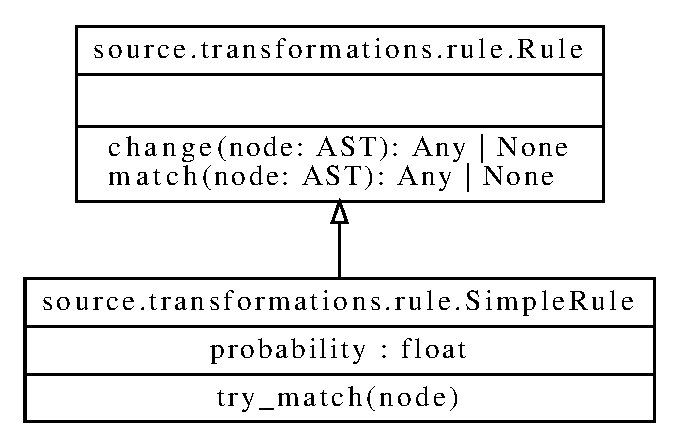
\includegraphics[width=0.6\textwidth]{images/uml/SimpleRule.eps}
	\caption{A \emph{SimpleRule} osztály}
	\label{fig:SimpleRule}
\end{figure}

Az \emph{In-place} az AST egy node-ját alakítják át,
ha azon a node-on sikeresen mintaillesztettek, vagyis a node-ot helyben változtatják.

Ezek az általam implementált legegyszerűbb szabályok,
az \emph{Rule}-tól örökölt \emph{match} metódust definiálva mintaillesztenek egy node-ra.
A mintaillesztés sikerességének jelentése az \emph{In-place} szabályoknál szabályfüggő.

Egyes szabályokban (pl. az \emph{InvertIf} szabályban) csak mintailleszteni kell a node-ra,
ezeknél a szabályoknál a \emph{match} visszatérési értéke \emph{bool} típusú
és a mintaillesztés sikerességére utal.

Más szabályokban (pl. a \emph{GuardDef} szabályban) megkönnyíti a dolgunkat,
ha a node-ot mintaillesztés közben "dekonstruáljuk", 
azaz a node bizonyos attribútumait vagy gyerekeit elmentjük és visszaadjuk,
hogy a \emph{change} metódus ezeket fel tudja használni.
Ezeknél a szabályoknál a \emph{match} visszatérési értéke \emph{None} típusú,
ha a mintaillesztés sikertelen.
Sikeres mintaillesztésnél a \emph{match} az elmentett attribútumokat vagy gyerekeket adja vissza
egy tuple-ben.

Ekvivalens és nem ekvivalens \emph{In-place} szabályokat is definiáltam.
Az ekvivalens szabályok
a \emph{rules\_eqv.rules\_simple} modulban,
a nem ekvivalens szabályok pedig
a \emph{rules\_neqv.rules\_simple} modulban
találhatóak.

Az \emph{In-place} szabályokban a \emph{change} metódus feladata a node átalakítása
és az átalakított node visszaadása.
A \emph{change} metódus először mintailleszt a \emph{try\_match} meghívásával.
A \emph{try\_match} visszatérési értéke alapján vagy átalakítja a node-ot,
vagy egy \emph{None} visszaadásával jelzi, hogy az adott node-ot nem tudja átalakítani.

Minden \emph{SimpleRule} osztályból származó szabály rendelkezik egy valószínüséggel változóval
(\emph{probability} a \ref{fig:SimpleRule}. ábrán).
Erre azért van szükség, mert a nagyon egyszerű szabályokat nem biztos,
hogy minden node-ra alkalmazni szeretnénk.
Ennek érdekében egy \emph{In-place} szabály létrehozásakor megadhatunk
egy 0 és 1 közötti valószínűséget, ami a szabály alkalmazásának valószínűsége.

A valószínűség implementációja miatt van szükség a \emph{try\_match} definiálására is.
Ez a metódus először mintailleszt a node-on.
Ha a mintaillesztés sikertelen, akkor leáll.
Ha a mintaillesztés sikeres,
akkor generál egy 0 és 1 közötti számot,
amivel a valószínűséget szimulálja.
Ha a generált szám kisebb mint a szabály valószínűsége,
akkor a mintaillesztést sikeresnek tekintjük, különben sikertelennek.

Az \emph{In-place} szabályokat
a \emph{RuleTransformer} osztályból származó \emph{TSimple} osztály alkalmazza.
A \emph{TSimple} osztály UML diagramját a \ref{fig:TSimple}. ábrán láthatjuk.

\begin{figure}[H]
	\centering
	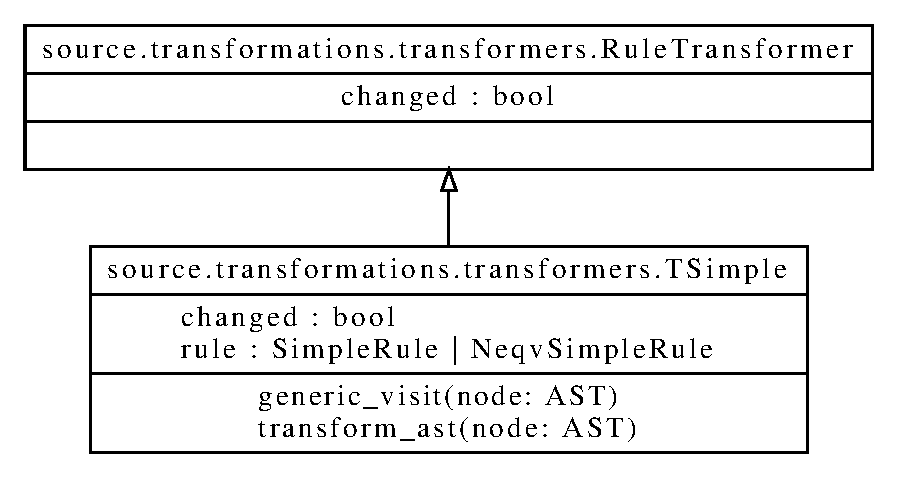
\includegraphics[width=0.6\textwidth]{images/uml/TSimple.eps}
	\caption{A \emph{TSimple} átalkító osztály}
	\label{fig:TSimple}
\end{figure}

A \emph{TSimple} működése egyszerű,
a \emph{generic\_visit}-et felülírva mélységi bejárással meglátogatja az AST node-jait.
Minden meglátogatott node-ra alkalmazza
a \emph{rule} példány szintű változóban található szabályt.
Ha a szabály alkalmazható, akkor a node-ot átalakítja, különben változatlanul hagyja.
A bejárást a \emph{transform\_ast} indítja.
A bejárás végén az eredmény a \emph{changed} bool-ban található,
ami azt jelzi, hogy sikerült-e a szabályt legalább egyszer alkalmazni az AST-n.

Az \emph{In-place} szabályok listáját a \ref{tab:in-place-rules-eqv}. és \ref{tab:in-place-rules-neqv}.
táblázatokban láthatjuk.
\footnote{\textbf{p} a szabályok alap valószínűsége}

\begin{center}
	\begin{longtable}{ | p{0.25\textwidth} | p{0.6\textwidth} | p{0.05\textwidth} | }
		\hline
		\multicolumn{3}{|c|}{\textbf{Ekvivalens in-place szabályok}}
		\\ \hline
		
		\textbf{Szabály} & \textbf{Magyarázat} & \textbf{p}
		\\ \hline \hline
		\endfirsthead % első oldal fejléce
		
		\hline
		\textbf{Szabály} & \textbf{Magyarázat} & \textbf{p}
		\\ \hline \hline
		\endhead % többi oldal fejléce
		
		\hline
		\endfoot % többi oldal lábléce
		
		\endlastfoot % utolsó oldal lábléce
		
		\emph{MultipleAssign}
		& Többszörös értékadást több értékadássá alakító szabály
		& 1.0
		\\ \hline

		\emph{TupleAssign}
		& Tuple értékadást több értékadássá alakító szabály
		& 1.0
		\\ \hline

		\emph{GuardDef}
		& Függvény else ágbeli return utasítását early return utasítássá alakító szabály
		& 1.0
		\\ \hline

		\emph{SingleIf}
		& \textbf{if} utasításon belül található \textbf{if} utasítás feltételének hozzáadása a külső \textbf{if} feltételéhez
		& 1.0
		\\ \hline
		
		\emph{InvertIf}
		& \textbf{if} utasítást \textbf{if} és \textbf{else} ágait megfordító szabály
		& 1.0
		\\ \hline

		\emph{DeMorgan}
		& De Morgan azonosságokat alkalmazó szabály
		& 1.0
		\\ \hline

		\emph{DoubleNegation}
		& Dupla negációkat eltütető szabály
		& 1.0
		\\ \hline

		\emph{BetterNegation}
		& Külső negációkat bevivő szabály
		& 1.0
		\\ \hline

		\emph{CommutativeMult}
		& Szorzás jobb és bal operandusát felcserélő szabály
		& 0.5
		\\ \hline

		\emph{ShuffleKeywords}
		& Keyword argumentumokat összekeverő szabály
		& 0.66
		\\ \hline

		\emph{InsertContinue}
		& \textbf{continue} utasítás beszúrása a ciklus végére
		& 0.11
		\\ \hline

		\emph{InsertPass}
		& \textbf{pass} utasítás beszúrása egy függvény definícióba
		& 0.11
		\\ \hline

		\caption{Ekvivalens \emph{In-place} szabályok táblázata}
		\label{tab:in-place-rules-eqv}
	\end{longtable}
\end{center}

\begin{center}
	\begin{longtable}{ | p{0.25\textwidth} | p{0.6\textwidth} | p{0.05\textwidth} | }
		\hline
		\multicolumn{3}{|c|}{\textbf{Nem ekvivalens in-place szabályok}}
		\\ \hline
		
		\textbf{Szabály} & \textbf{Magyarázat} & \textbf{p}
		\\ \hline \hline
		\endfirsthead % első oldal fejléce
		
		\hline
		\textbf{Szabály} & \textbf{Magyarázat} & \textbf{p}
		\\ \hline \hline
		\endhead % többi oldal fejléce
		
		\hline
		\endfoot % többi oldal lábléce
		
		\endlastfoot % utolsó oldal lábléce
		
		\emph{NeqvNegateIf}
		& \textbf{if} feltételének negálása ágak megfordítása nélkül
		& 0.5
		\\ \hline

		\emph{NeqvInvertIf}
		& \textbf{if} ágainak megfordítása feltétel negálása nélkül
		& 0.5
		\\ \hline

		\emph{NeqvInsertBreak}
		& \textbf{break} utasítás beszúrása ciklus elejére
		& 0.33
		\\ \hline

		\emph{NeqvInsertContinue}
		& \textbf{continue} utasítás beszúrása ciklus elejére
		& 0.33
		\\ \hline

		\emph{NeqvInsertReturn}
		& \textbf{return} utasítás beszúrása ciklus elejére
		& 0.33
		\\ \hline
		
		\emph{NeqvSwapAndOr}
		& \textbf{and} és \textbf{or} operátorok felcserélése
		& 0.5
		\\ \hline

		\emph{NeqvSwapAddSub}
		& + és - operátorok felcserélése
		& 0.5
		\\ \hline

		\emph{NeqvReplaceNums}
		& Szám konstansokat átíró szabály
		& 0.33
		\\ \hline

		\caption{Nem ekvivalens \emph{In-place} szabályok táblázata}
		\label{tab:in-place-rules-neqv}
	\end{longtable}
\end{center}

\subsection{\emph{For} szabályok}

A \emph{For} szabályok a \emph{transformations} csomag legösszetettebb szabályai.
Ezek a szabályok for ciklussal megadott alap programozási tételek megoldásából
(pl. összegzés vagy kiválogatás), Python specifikus, comprehension kifejezést használó
megoldásokat állítanak elő.

A comprehension egy speciális kifejezés a Python absztrakt-nyelvtanában, ami
egy iterálható kifejezéstből (iter), egy target-kifejezésből (target)
és "if" kifejezések listájából (ifs) áll.

Az "if" kifejezések a nyelvtan definíciójában kifejezések nem if statement-ek.
Comprehension kifejezést használhatunk alap
mutable adatstruktúrák (list, dict, set) vagy generátorok meghatározására.

Egy \emph{For} átalakítás személtetéséhez tekintsük a következő feladat példáját:

\newtheorem{example}{Példa}
\begin{example}
Adjuk meg az $xs: Iterable$, azon elemeit egy listában,
amikre a $condition$ függvény teljesül
(feltéve, hogy $bool(condition(x))$ az $xs$ minden $x$ elemére értelmes).
\end{example}

Az egyik megoldás, ha létrehozunk egy üres listát,
majd egy for ciklussal iterálunk az $xs$-en és
a listához adjuk azokat az elemeket amelyekre a $condition$ függvény
"truthy" értéket ad vissza.

A másik megoldás, ha a listát egy list comprehensionnel adjuk meg,
ekkor a for ciklus if feltételét a list comprehension végére tesszük.

\noindent
\begin{minipage}[t]{.48\textwidth}
\lstset{
	caption={Példa megoldása for ciklussal},
	label=src:forSolution,
	numbers=none
}
\begin{lstlisting}[language={Python}]
	result = []
	for x in xs:
		if condition(x):
			result.append(x)
\end{lstlisting}
\end{minipage}
\hfill
\begin{minipage}[t]{.48\textwidth}
\lstset{
	caption={Példa megoldása comprehensionnel},
	label=src:compSolution,
	numbers=none
}
\begin{lstlisting}[language={Python}]
	result = [
		x for x in xs
		if condition(x)
	]
\end{lstlisting}
\end{minipage}

Pythonban a legtöbb esetben a második megoldás a preferált az elsővel szemben,
rövidebb és általában olvashatóbb is.

A \emph{For} szabályok célja a példához hasonló átalakítások megvalósítása.
Ekvivalens és nem ekvivalens \emph{For} szabályokat is implementáltam.
A szabályok egy értékadást és egy for ciklust alakítanak comprehensionös kifejezéssé.
A szabályok közt vannak list, dict és set comprehensionné alakító szabályok,
illetve számok össszegének és feltételes összegének kiszámítására is van egy szabály.

A \emph{For} szabályok a sablonfüggvény (\emph{template method})
tervezési minta segítségével működnek.
A mintaillesztést a \emph{ForRule} osztály \emph{match} metódusa végzi.
A \emph{match} metódus a sablonfüggvény,
a sablonfüggvény lépései pedig
a \emph{match\_Assign} és \emph{match\_For} metódusok.

\begin{figure}[H]
	\centering
	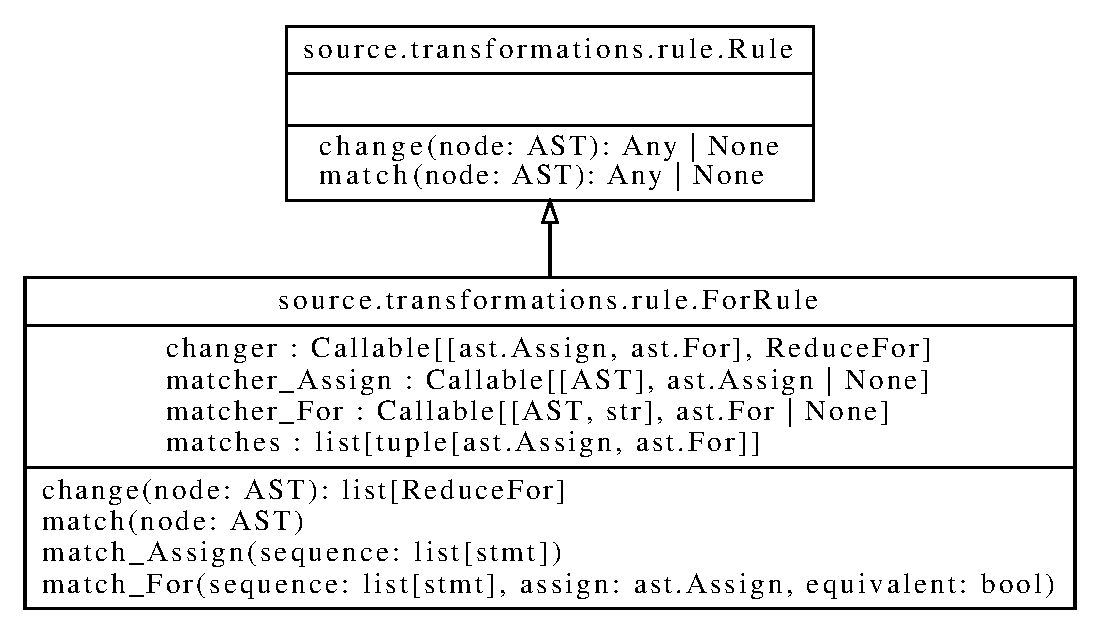
\includegraphics[width=0.6\textwidth]{images/uml/ForRule.eps}
	\caption{\label{fig:ForRule}A \emph{ForRule} osztály}
\end{figure}

A \ref{fig:ForRule}. ábrán látható
\emph{matcher\_Assign} és \emph{matcher\_For} osztályszintű változók függvények.
Ezeket a függvényeket használom a
\emph{match\_Assign} és \emph{match\_For}-ban az \emph{Assign} és \emph{For}
node-ok mintaillesztésére.

A mintaillesztésénél a statement listát tartalmazó node-okra kell mintailleszteni,
ezek a Python absztrakt-nyelvtanának megfelelően azok a node-ok,
amik \emph{body}, \emph{orelse} vagy \emph{finalbody} attribútumokat tartalmaznak.

Az ilyen node-okat három \texttt{match} utasítással ismerehetjük fel,
amik a következő esetekre mintaillesztenek:

\lstinline{AST(body=[_, _, *_])},
\lstinline{AST(orelse=[_, _, *_])},
\lstinline{AST(finalbody=[_, _, *_])}.

Ha a node-ban van statementek listáját tartalmazó attribútum,
akkor arra az attribútumra meghívjuk a \emph{match\_Assign} metódust.

A \emph{match\_Assign} először a statementek listájában szereplő
node-okra meghívja a \emph{matcher\_Assign} függvényt.
Ha a \emph{matcher\_Assign} sikeresen mintailleszt a node-ra,
akkor a listában az utána szereplő
statementeken kell mintailleszteni a \emph{matcher\_For} segítségével.
Ha a \emph{matcher\_For} is sikeresen mintaillesztett akkor az átalakítást
el lehet végezni
a felismert \emph{Assign} és \emph{For} node-okon.
Ilyenkor az átalakítást a felismert \emph{Assign} és \emph{For} párokat tartalmazó
\emph{matches} listához adjuk.

A \emph{For} átalakítások felismerésének pszeudokódját a
\ref{alg:forMatchAlgorithm}. algoritmuson láthatjuk.

\begin{algorithm}[H]
	\caption{A \emph{For} átalakítások felismerésének algoritmusa}
	\label{alg:forMatchAlgorithm}
	\textbf{\underline{method}} ForRule::match\_Assign($statements: list[stmt]$)
	
	\begin{algorithmic}[1]
	\State $n$ := length$(statements) - 1$
	\For {$i$ \textbf{in} $0 \ldots n$}
		\State $assign$ := self.matcher\_Assign($statements[i]$)
		\If {$assign$ \textbf{is not} None}
			\State self.match\_For($statements[i+1:n]$, $assign$)
		\EndIf
	\EndFor
	\end{algorithmic}

	\textbf{\underline{method}} ForRule::match\_For($statements: list[stmt]$, $assign: Assign$)
	\begin{algorithmic}[1]	
	\State $name$ := $assign$.target.id
	\For {$statement$ \textbf{in} $satements$}
		\State $matched\_for$ := self.matcher\_For($statement$, $name$)
		\If {$matched\_for$ \textbf{is not} None}
			\State self.matches.append(($assign$, $matched\_for$))
			\State \Return
		\EndIf
		\If {set(ids($statement$)) $\cap$ set(ids($assign$)) $\neq \emptyset$}
			\State \Return
		\EndIf
	\EndFor
	\end{algorithmic}
\end{algorithm}

Ha az \ref{alg:forMatchAlgorithm}. algoritmus lefutott,
akkor a megfelelő \emph{Assign} és \emph{For} node
párokat a szabály \emph{matches} listájában találhatjuk meg.

A \emph{For} szabályok \emph{change} függvénye először előállítja a \emph{matches} listát.
Ha a \emph{matches} nem üres, akkor az elemeiből létrehozza és visszaadja
a változtatásokat egy listában ami \emph{ReduceFor} példányokat tartalmaz
(lásd \emph{change} metódus a \ref{fig:ForRule}. ábrán).

A \emph{ReduceFor} osztály egy példánya tartalmazza
a törlendő \emph{Assign} node-ot,
a generált comprehension node-ot
és a \emph{For} node-ot, amit helyettesíteni kell a generált node-al.

A \emph{For} szabályokat a \emph{TFor} átalakító osztály segítségével lehet alkalmazni.
Az átalakítások alkalmazásához az átalakító osztálynak kétszer kell bejárnia az AST-t.

Az első bejárással összegyűjtük a lehetséges változtatásokat az AST node-jain.
A változásokat a \emph{TFor} osztály \emph{results} listájában tároljuk
(lásd \ref{fig:TFor}. ábra).
A lista mindig a szabály \emph{change} metódusa által visszaadott
\emph{ReduceFor} példányokkal bővül.

Az első bejárás után a lehetséges változtatások már a \emph{results} listában vannak.
Az AST-t újból bejárva a változtatásokat elvégezzük.
A megjelölt \emph{Assign} node-okat töröljük
és megjelölt \emph{For} node-okat a generált kifejezésre változtatjuk.

\begin{figure}[H]
	\centering
	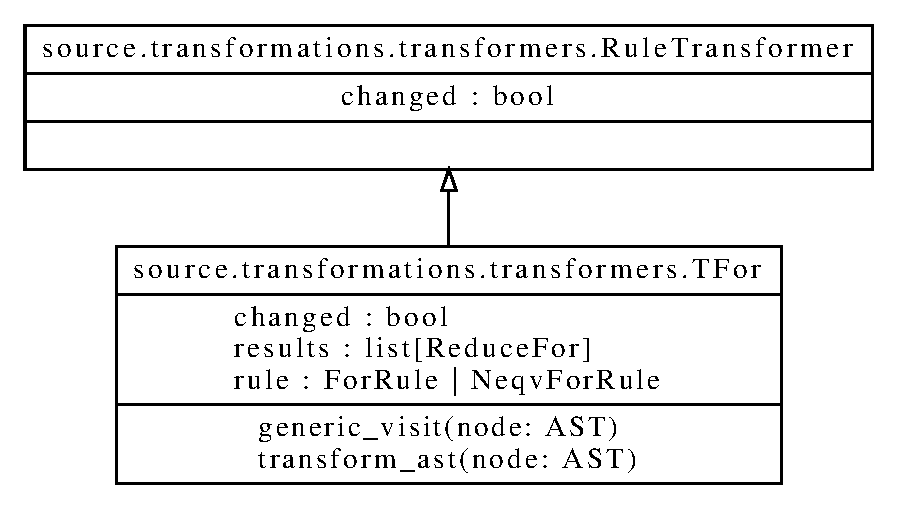
\includegraphics[width=0.6\textwidth]{images/uml/TFor.eps}
	\caption{\label{fig:TFor}A \emph{TFor} átalakító osztály}
\end{figure}

A \emph{TFor} osztály \emph{transform\_ast} metódusa kétszer hívja
meg a \emph{visit}-et a paraméterül kapott node-ra.
A bejárást az ozstály a \emph{generic\_visit} felülírásával végzi.

A \emph{transformations} csomagban négy féle \emph{For} szabályt implementáltam.
Az első három szabály az üres dict, list vagy set -et inicializáló for ciklusokat,
alakítja dict, list vagy set comprehensionné (a feltételes esetet is vizsgálva).

A negyedik szabály a nullával inicializált, for ciklus által számolt,
összeget vagy feltételes összeget alakítja
egy \emph{sum} builtin függvény hívássá.

Mind a négy fajta \emph{For} szabálynak van ekvivalens és nem ekvivalens változata is.
A különböző szabályok fajtáit a \ref{fig:ForRules}. ábrán látható osztálydiagrammon láthatjuk.

\begin{figure}[H]
	\centering
	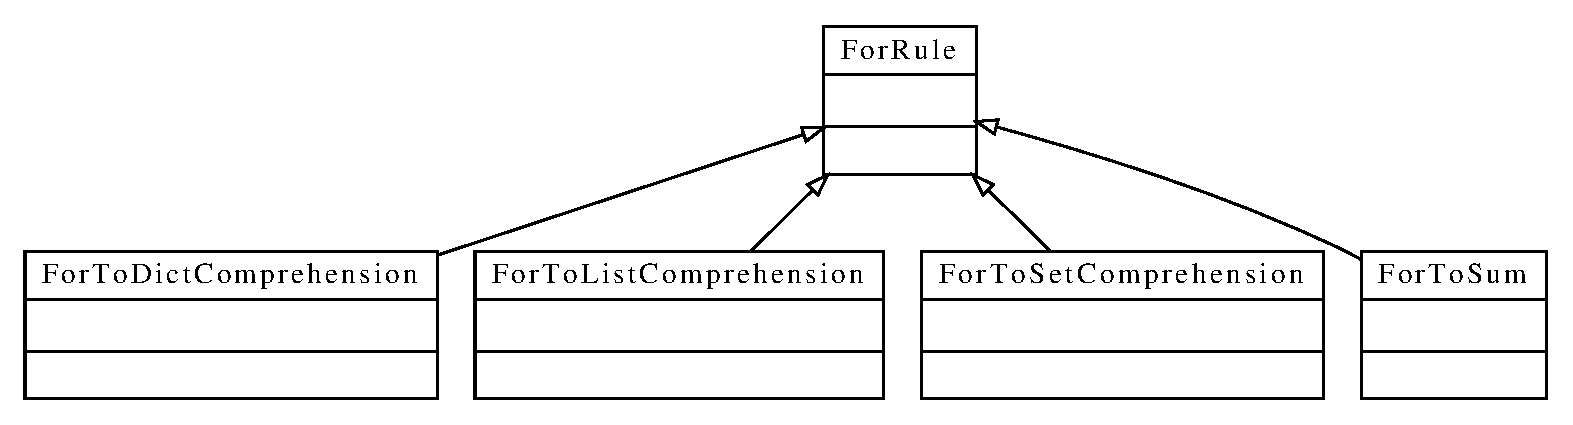
\includegraphics[width=0.8\textwidth]{images/uml/ForRules.eps}
	\caption{\label{fig:ForRules}A \emph{For} szabályok UML diagramja}
\end{figure}

\pagebreak

\subsection{API az átalakítások alkalmazásához}

Az átalakításokat a \emph{transformation} modul segítségével alkalmazhatjuk.
A modul célja egy olyan API létrehozása amivel könnyen átalakíthatunk kódokat vagy kódok AST-jét.
Az API implementálásához az absztrakt gyár (\emph{Abstract factory}) és az építő (\emph{Builder})
tervezési mintákat használtam fel.

Ahogy azt az előző fejezetekben részleteztem
egy szabály alkalmazásához két objektumot kell létrehozni:
a szabályt és az annak megfelelő átalakító osztályt.
Az absztrakt gyár az átalakító osztályok és szabályok példányosításában segít.

Az absztrakt gyár mintát a \emph{create\_rule} függvény implementálja.
A függvény a szabálytípusok átalakító osztályait állítja párba a szabályokkal.
Egy szabálynév alapján a \emph{create\_rule} létrehozza
a szabálynak megfelelő átalakító osztály példányát.
Ha a megadott nevű szabály nem létezik, akkor \emph{ValueError} exceptiont dob.

Egy AST-t az átalakítás során gyakran több átalakító osztállyal is be szeretnénk járni.
Például ha két szabályt szeretnénk alkalmazni, akkor az AST-t kétszer kell bejárni.
A többszörös bejárások elvégzésében az építő tervezési mintát megvalósító
\emph{TransformationBuilder} osztály segít.

A \emph{TransformationBuilder} osztály segítségével
létrehozhatjuk átalakítók listáját, amivel egy AST-n több egymás utáni átalakítást
(például szabályokat) hajthatunk végre.
Ehhez definiáltam a \emph{Transformer} interfészt, amit minden átalakítónak
implementálnia kell.
A \emph{Transformer} interfészben csak egy metódus található, a \emph{transform\_ast},
ami az AST bejárását és átalakítását végzi.
Ezt a metódust implementálják a szabályok átalakító osztályai is.

Az is gyakran előfordul, hogy nem az eredeti AST-t akarjuk átalakítani, hanem annak egy másolatát,
erre a célra a \emph{CopyTransformer} osztályt használhatjuk.
A \emph{CopyTransformer} osztályt egy AST alapján példányosíthatjuk.
A megadott AST-t a \emph{CopyTransformer} lemásolja a \emph{deepcopy} segítségével.
Az átalakításokat már a másolaton végzi a \emph{TransformationBuilder}-t felhasználva.

\pagebreak

\section{A \emph{client} csomag}

A \emph{client} csomag feladata az adatbáziskapcsolat és az indexek létrehozása.
A kliens a \emph{pymongo} könyvtárat használja, implementációja a \emph{Client} osztályban van.
Ha a szoftvernek az adatbázisra van szüksége azt ezen az osztályon keresztül érheti el.
Például az adatbázis forráskódokat és forráskód-párokat tartalmazó kollekciói a kliensen
keresztül elérhetők.

A \emph{Client} osztály a Python-ban gyakori \emph{monostate} \cite{monostatePattern}
tervezési mintát használja, a minta a \emph{singleton}-hoz hasonló,
de több példány létrehozását is megengedi.
Egy \emph{monostate} osztálynak van egy belső (statikus) állapota,
példányosításnál ezt a belső állapotot adja vissza.
Ez hasznos, mert a példányok egy közös állapoton osztoznak, ami a program több részéről is elérhető.

Python-ban az objektumok állapota reprezentálható egy dict segítségével,
ezért a \emph{monostate} mintát nagyon egyszerű implementálni:
a belső állapot egy dict lesz, példányosításnál a belső állapot dict-je alapján hozunk létre egy objektumot.

\begin{figure}[H]
	\centering
	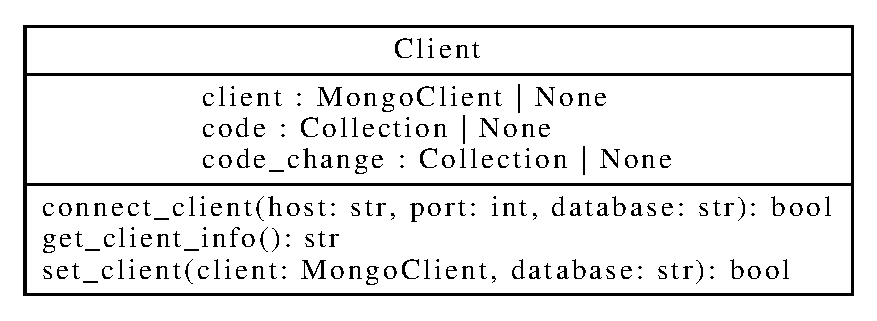
\includegraphics[width=0.6\textwidth]{images/uml/Client.eps}
	\caption{A \emph{Client} osztály UML diagramja}
\end{figure}

Amikor először példányosítunk a \emph{Client}-ből a \emph{client}, \emph{code} és \emph{code\_change}
attribútumai \emph{None} értékeket vesznek fel (ez a kezdelteges belső állapot).

Ha ezután meghívjuk a \emph{connect\_client} metódust az adatbázis paramétereivel
és a kapcsolat 10 másodpercen belül létrejön, akkor a kapcsolat sikeres.
Ekkor
a \emph{client} attribútum az adatbáziskliens,
a \emph{code} és \emph{code\_change} attribútumok pedig rendre
a kódokat és kód-párokat tartalmazó kollekciók lesznek.

A kollekciók akkor is létrejönnek a kliens szintjén ha az adatbázisban még nem szerepelnek.
Ebben az esetben a kollekció az adatbázisban akkor jön létre, ha a kliensen keresztül elmentünk egy dokumentumot.
A kliens a szükséges indexeket is definiálja az adatbázisban.

\section{A \emph{model} csomag}
\label{sec:model}

A \emph{model} csomag a feladata a forráskód-párok modellezése, három modulból áll:

\begin{itemize}
	\item \emph{datatypes} - az adattípusokat definiáló modul
	\item \emph{serializers} - az adattípusokat szerializáló modul
	\item \emph{stores} - az adattípusokat elmentő modul
\end{itemize}

A csomagban két adattípust definiáltam: a \emph{Code} és \emph{CodeChange} típusokat.
A \emph{Code} a forráskódok modellje, a \emph{CodeChange} pedig a forrráskód-párokat modellezi.
Az adatokat modellező osztályok UML diagramjait a \ref{fig:model}. ábrán láthatjuk.

\begin{figure}[H]
	\centering
	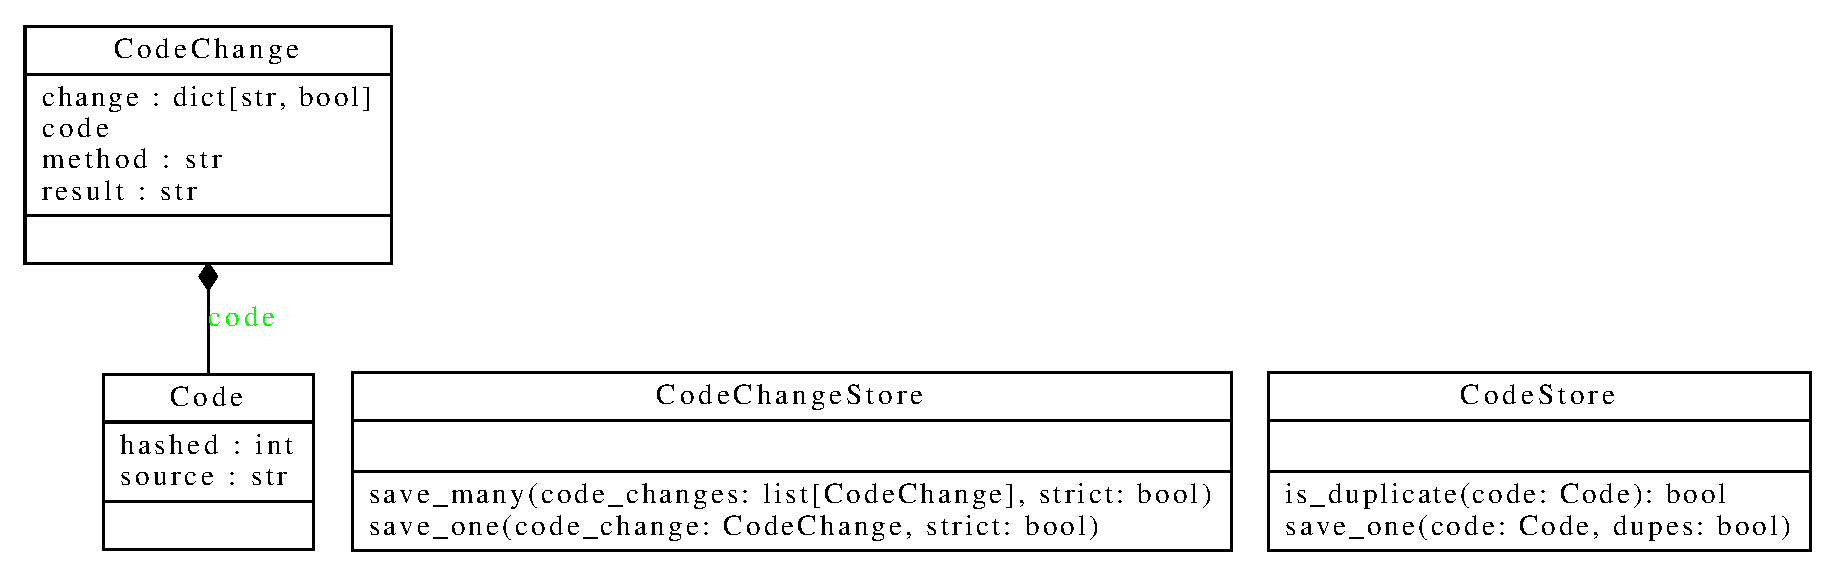
\includegraphics[width=0.9\textwidth]{images/uml/models.eps}
	\caption{\label{fig:model}A model csomag osztályainak UML diagramjai}
\end{figure}

A forráskód a duplikátumok kiszűrése miatt rendelkezik saját modellel.
A duplikált forráskódok szűrése azért szükséges, mert GitHub-on a kódok jelentős része duplikátum
\cite{GitHubDuplication},
vagyis ha GitHub-ról bányászunk kódokat akkor a generált adathalmaz minőségén javíthatunk,
a duplikátumok kiszűrésével.

A kódok modellje ezért a kód mellett a kód \emph{sha256}-os hashét is tárolja.
Mielőtt a kódot elmentjük az adatbázisba megnézzük, hogy a hash ütközik-e.

Ha nincs ütközés, akkor a kódot egyből a kollekcióhoz adhatjuk,
különben csak az ütköző kódokat kell összehasonlítani a duplikátumok kiszűréséhez.
A hash attribútuma indexelve van a kódokat tartalmazó kollekcióban,
ez biztosítja a gyors lekérdezést.

A \emph{CodeStore} és \emph{CodeChangeStore} osztályokkal lehet a kódokat és kódpárokat
elmenteni az adatbázisba.
A duplikátumok szűrését a \emph{CodeStore} osztály \emph{save\_one} metódusa végzi.
A szűrés opcionális, ha nem szeretnénk szűrést azt a \emph{dupes} paraméterrel állíthatjuk be.


\section{Az \emph{app} csomag}

Az \emph{app} csomag feladata az átalakításokat szemléltető GUI-s alkalmazás megvalósítása.
Az alkalmazás architektúrája modell-nézet-kontroller (MVC) szerű.
Egy nézet rendelkezik egy kontrollerrel és a kontroller pedig egy modellel.

A nézet feladata a GUI definiálása és frissítése,
a modell feladata az adatelérés vagy az alkalmazás állapotának modellezése.
A kontroller ezt a két réteget köti össze,
így a nézet nem függ a modelltől és a modell sem a nézettől.

Az alkalmazás csomagjainak UML diagramját a \ref{fig:app_packages}. ábrán láthatjuk.

\begin{figure}[H]
	\centering
	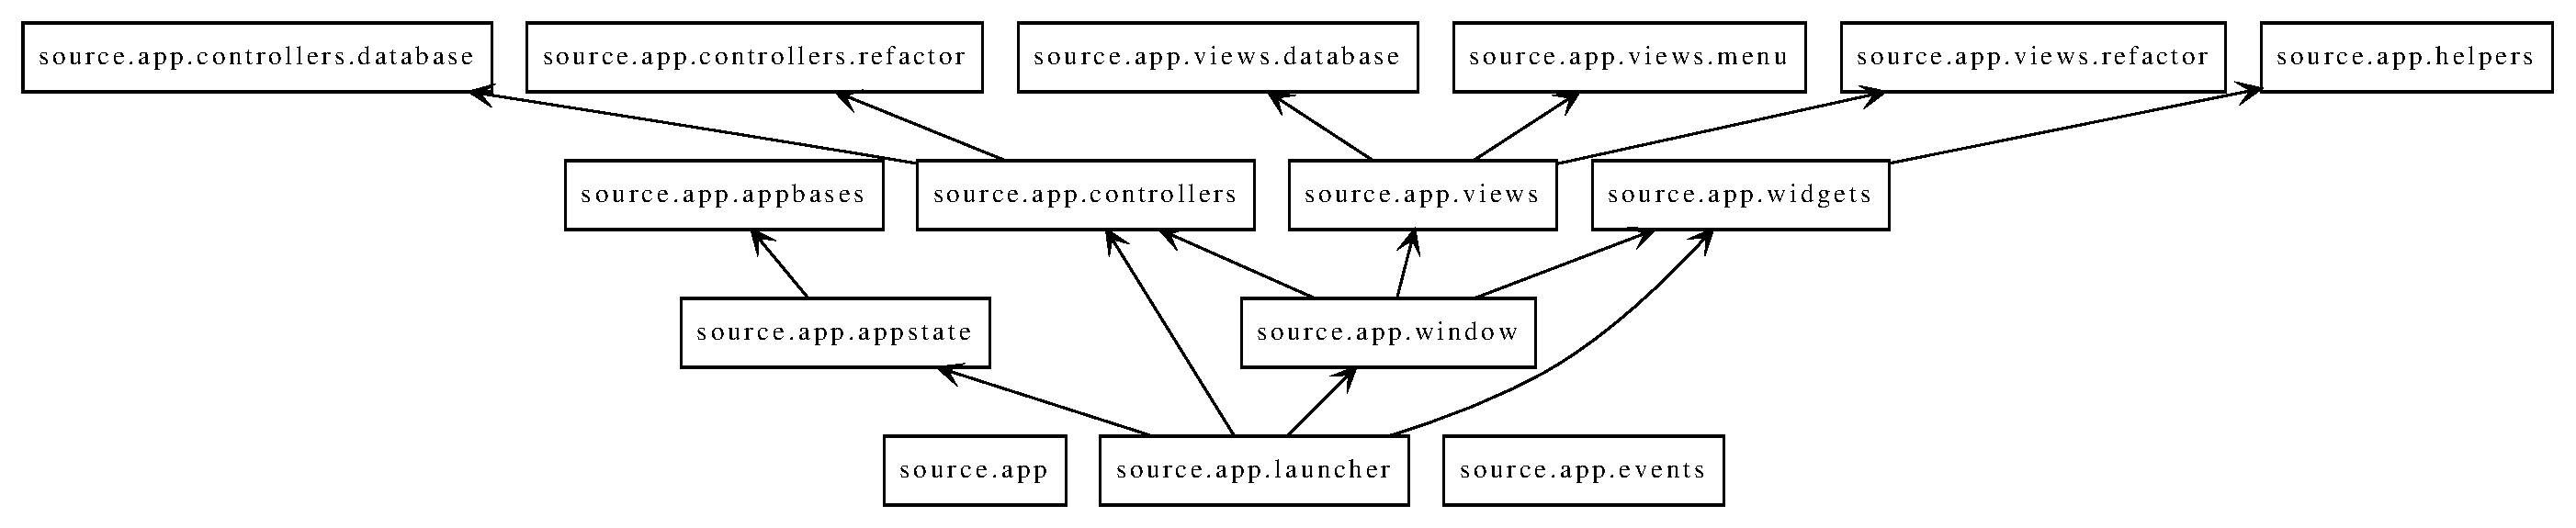
\includegraphics[width=0.9\textwidth]{images/uml/apppackages.eps}
	\caption{\label{fig:app_packages}Az alkalmazás csomagjai}
\end{figure}

\subsection{Állapotmodell}
\label{subsec:appstate}

Az alkalmazásban kétféle modell különböztethető meg:
az adatelérési modellek (lásd \ref{sec:model}. szekció),
és az alkalmzás állapotmodellje, ami az \emph{app.appstate} modul 
\emph{AppState} osztályában van definiálva.

Az állapotmodell a megfigyelő (\emph{observer}) tervezési mintát használja a nézetek frissítésére.
Az \emph{AppState} osztály az \emph{Observable} osztályból származik,
ezért rendelkezik megfigyelők dict-jével (\emph{observers}).
A megfigyelők dict-je tartalmazza az esemény-eseménykezelő key-value párokat.

Ha a nézet valamelyik komponenesét az állapotmodell egy változásának hatására szeretnénk frissíteni,
akkor azt az eseménykezelőt, ami frissíti,
hozzárendelhetjük az állapotmodell egy eseményéhez az \emph{app.events} modulból.

Hozzárendelni egy eseménykezelőt egy eseményhez az \emph{Observable} osztály
\emph{attach} metódusával lehet.
Ha az adott eseményt kiváltja egy változás a modellben, akkor a modell értesíti a
nézeteket,
vagyis az \emph{observers}-ben az eseményéhez rendelt eseménykezelőket meghívja,
a frissítéshez szükséges adatokat paraméterként továbbítva.

\begin{figure}[H]
	\centering
	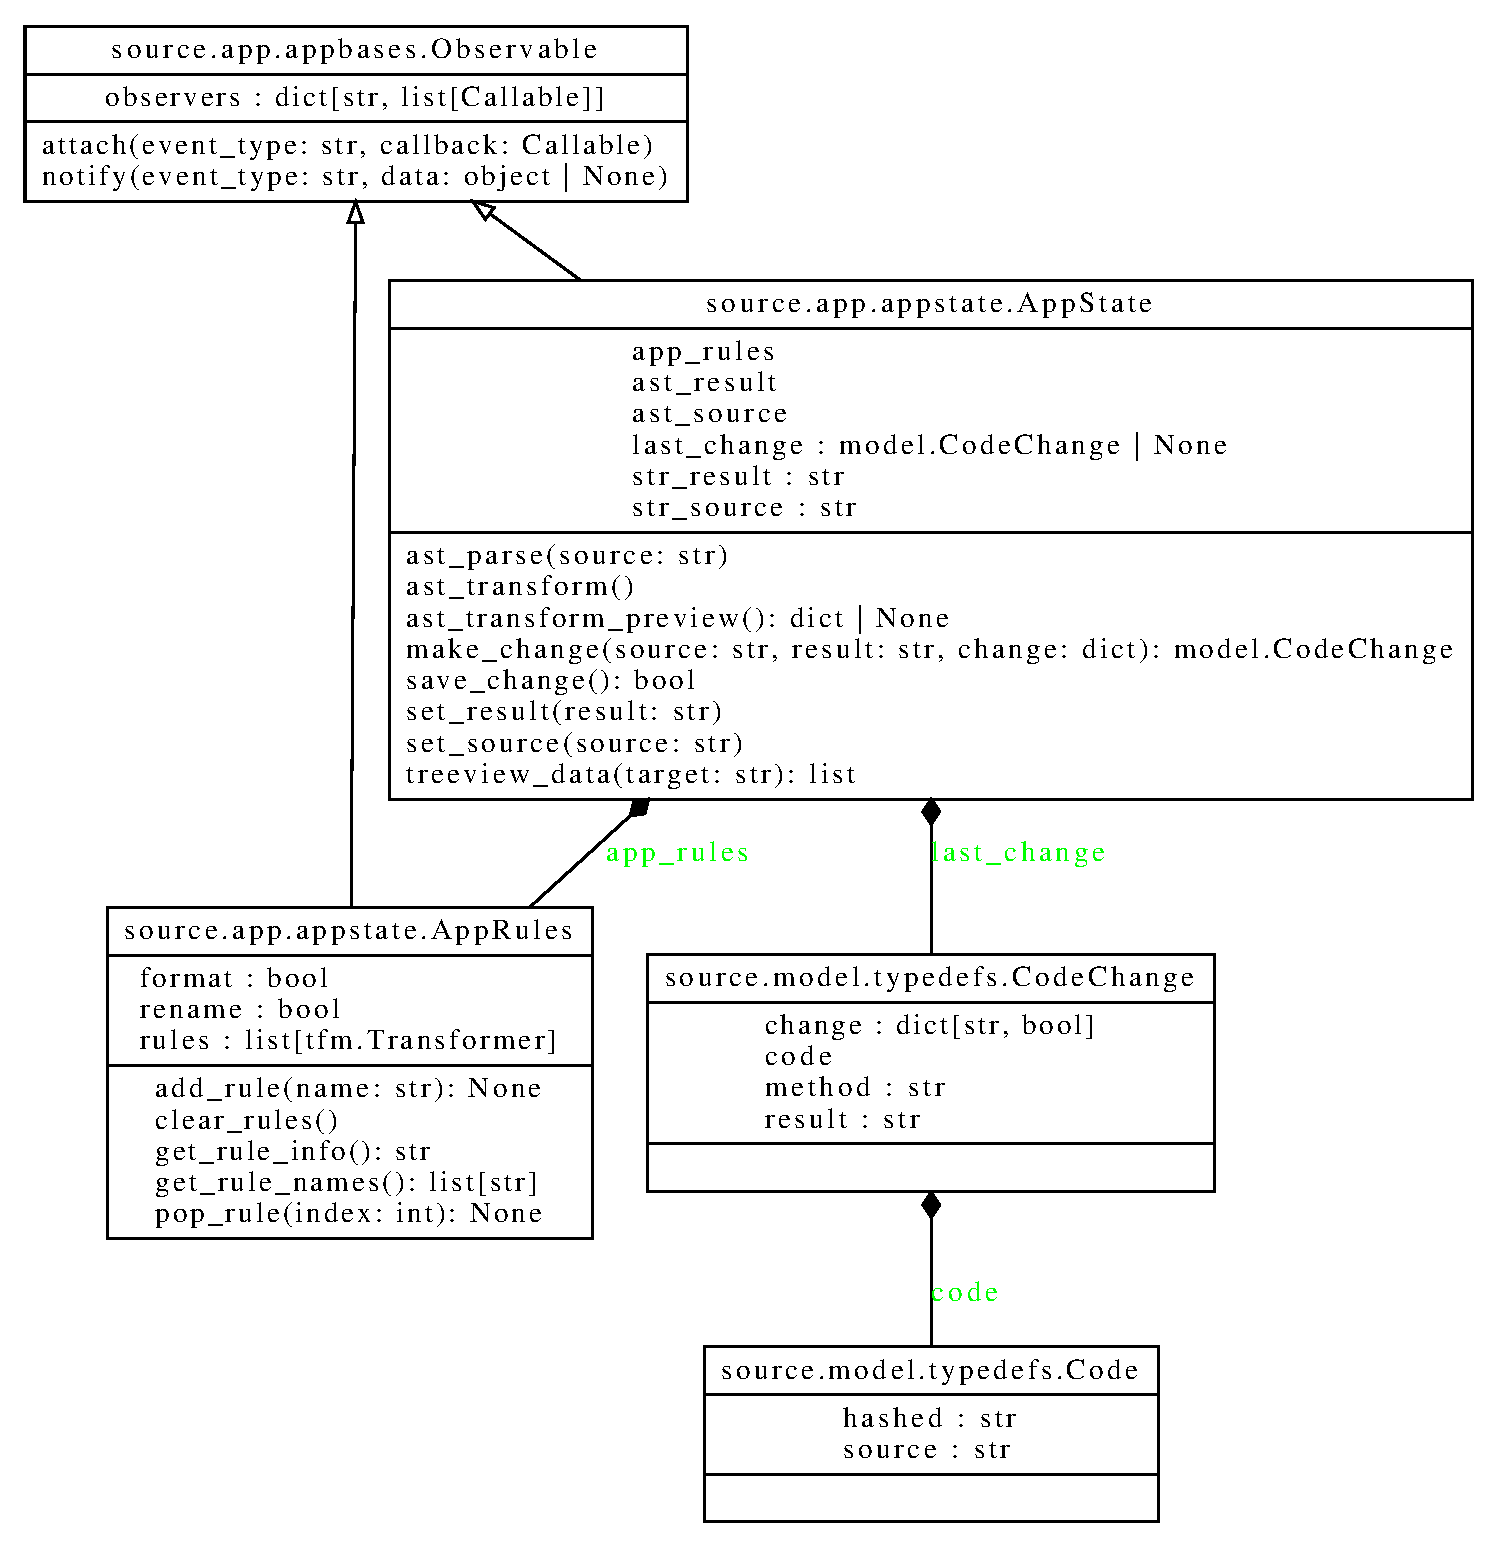
\includegraphics[width=0.9\textwidth]{images/uml/appstate.eps}
	\caption{\label{fig:AppState}Állapotmodell és kapcsolódó osztályok UML diagramjai}
\end{figure}

Az állapotmodel UML diagramját a \ref{fig:AppState}. ábrán látjhatjuk.
Az alkalmazás egy állapotát a bemeneti és kimineti AST-k, az ezekből generált kódok,
az átalakításért felelő szabályok listája, és az utolsó átalakítás írják le.

Az AST-k és a belőlük generált kódok az \emph{AppState} osztály példány szintű változói.
Ezeken kívül az állapotmodell az \emph{AppRules} és a \emph{CodeChange} osztályok egy-egy
példányát
is tartalmazza, ezek rendre az átalakításért felelő szabályokat és az utolsó átalakítást
tárolják.

Az \emph{AppRules} a szabályok állapotát modelezi, szintén az \emph{Observable}-ből
származik.
Ez az osztály tartalmazza a kiválasztott szabályokat a \emph{rules} listában,
a \emph{format} és \emph{rename} bool-okkal pedig azt tárolja, hogy az átalakított
kódot kell-e formatálni és hogy az átnevezéseket végre kell-e hajtani.

\pagebreak

Az utolsó validált átalakítást a \emph{CodeChange} osztály egy példánya tárolja.
Ahogy azt az előző szekcióban is említettem ezzel az osztállyal,
lehet elmenteni átalakításokat az adatbázisba.

A modellt az \emph{AppState} metódusai segítségével változtathatjuk.
A metódusok az AST-k átalakításáért és az utolsó átalakítás mentéséért felelnek,
a modellel kapcsolatos eseményeket is ezek váltják ki.

\subsection{Nézetek}

Az alkalmazás grafikus felhasználói felületének megvalósításához
a Python-ban alapból megtalálható
\emph{tkinter} könyvtárt használom, amit az erre építő \emph{ttkbootstrap} könyvtárral
egészítek ki.
A felhasználói felület forráskódja az \emph{app.views} csomagban és az \emph{app.widgets}
modulban található.

A \emph{tkinter} könyvtárban a GUI elemeket widgeteknek hívják.
Az applikáció widgetei az \emph{app.widgets} modulban vannak definiálja.
Például az \emph{app.widgets} modulban található
a Python szintaxis kiemelését támogató szövegdoboz
és az AST-ket ábrázoló fa-nézet definíciója is.

Az applikáció összetettebb nézeteit az \emph{app.views} csomagban definiáltam.
Ezek a nézetek szintén widgetek,
de az \emph{app.widgets} widgeteivel ellentétben
rendelkeznek egy kontrollerel,
amit a modellel való kommunikációhoz használnak
(az \emph{app.widgets} widgetei nem férnek hozzá a modellekhez).

Az \emph{app.view} widgetei az \emph{app.appbases.View} osztályból származnak.
A \emph{View} osztály egy \emph{tkinter}-es frame, ami
a nézethez tartozó kontroller példányával jön létre.
Az alkalmazásban három ilyen kontrollerrel rendelkező nézet van,
ezek osztálydiagrammjait a \ref{fig:views}. ábrán láthatjuk.

\begin{figure}[H]
	\centering
	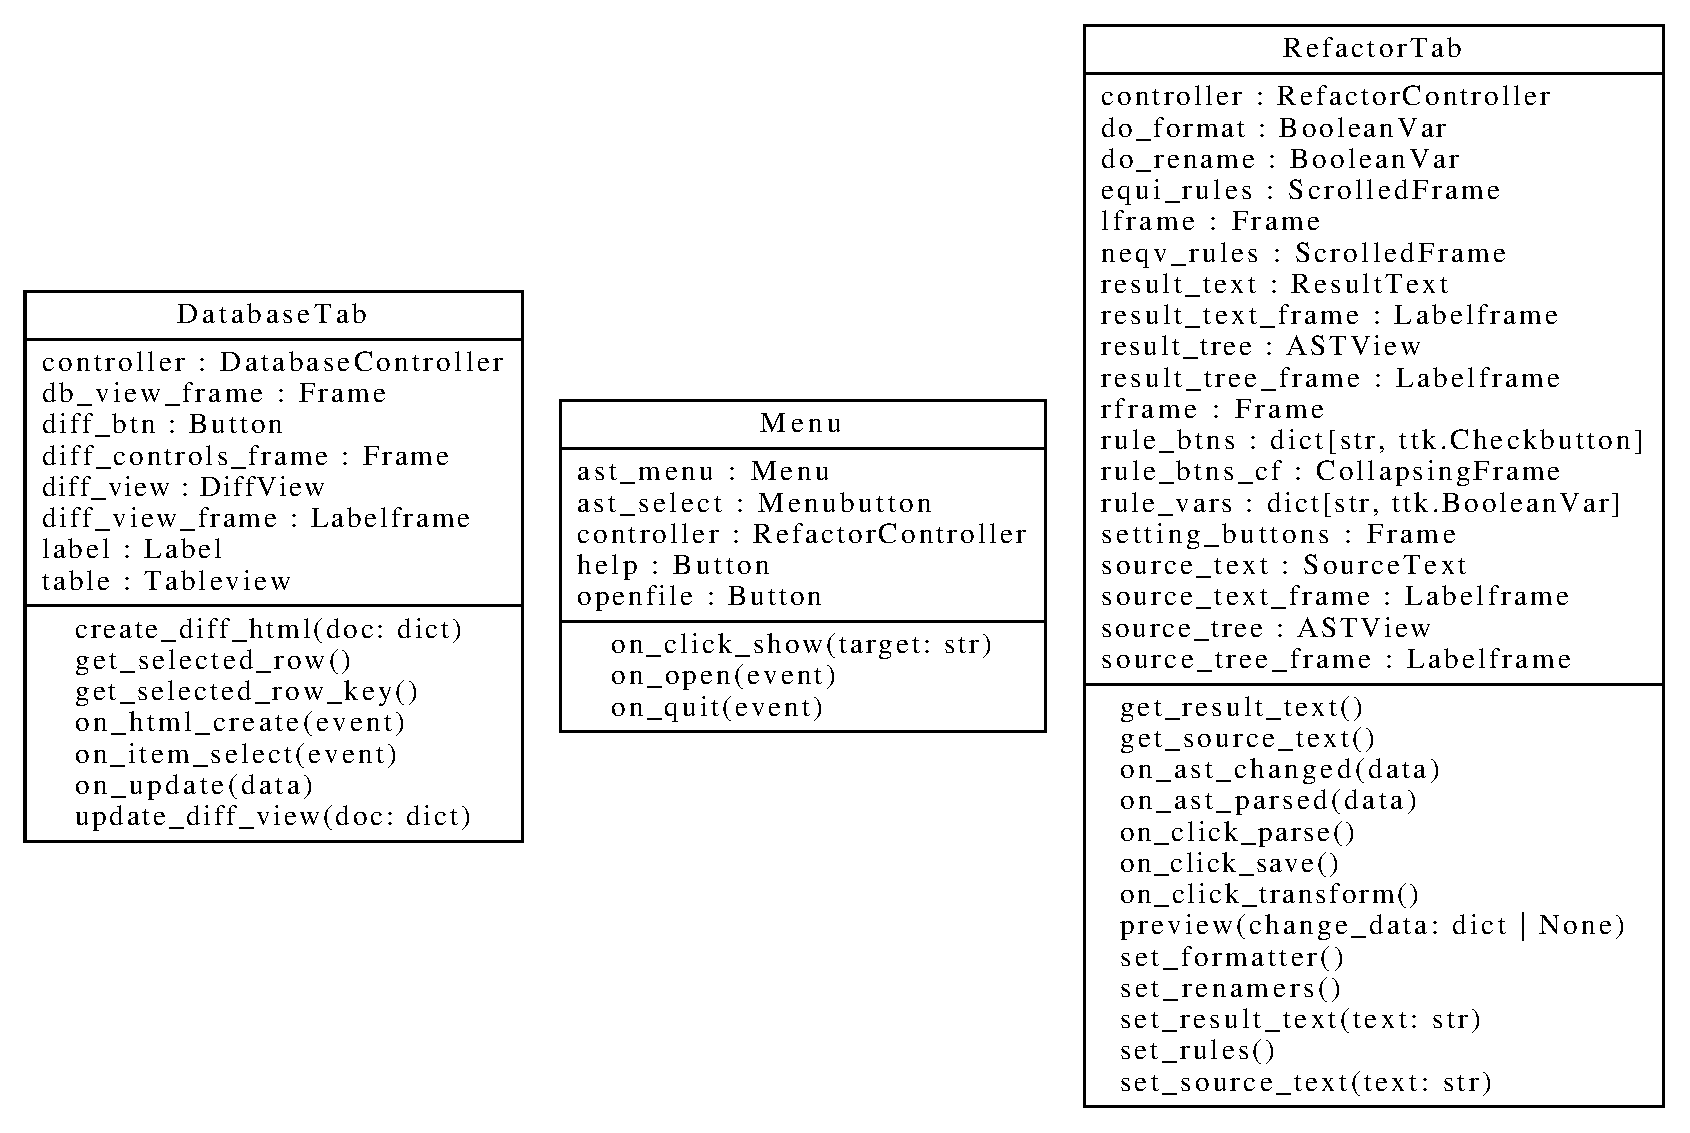
\includegraphics[width=0.9\textwidth]{images/uml/views.eps}
	\caption{\label{fig:views}A nézetek osztálydiagrammjai}
\end{figure}

\subsection{Kontrollerek}

A kontrollerek feladata a kommunikáció a modellek és nézetek között.
Ahogy azt a \ref{fig:views}. ábrán láthatjuk csak az alkalmazás
két fő nézete (\emph{DatabaseTab} és \emph{RefactorTab})
illetve a menü (\emph{Menu}) rendelkeznek kontrollerrel.

Az applikációban két különböző kontroller van.
A \emph{DatabaseController} az adatelérési modellekkel,
a \emph{RefactorController} az alkalmazás állapotmodelljével kommunikál.

\begin{figure}[H]
	\centering
	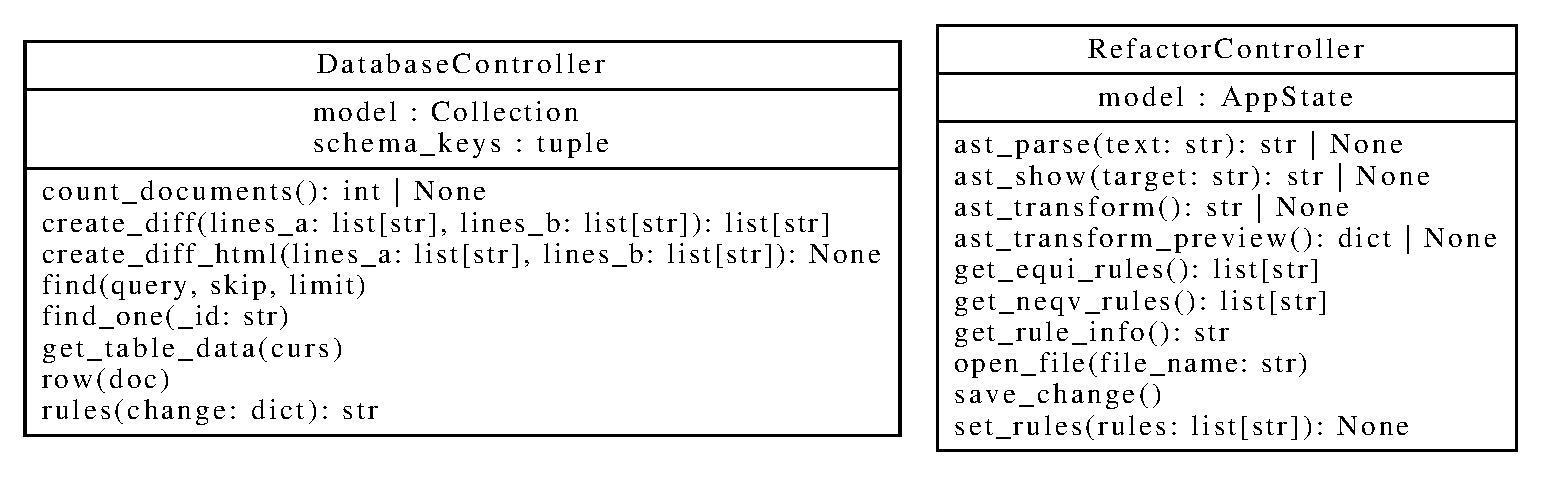
\includegraphics[width=0.9\textwidth]{images/uml/controllers.eps}
	\caption{\label{fig:controllers}A kontrollerek osztálydiagrammjai}
\end{figure}

Ha a nézeten olyan GUI esemény, történik aminek az eseménykezelője
a modell vagy az állapotmodell használatát igényli,
akkor az eseménykezelő a nézethez tartozó kontroller megfelelő metódusát hívja meg.
Ha az eseményhez input is tartozik (pl. egy szöveges doboz tartalma) akkor
azt is továbbítja a kontroller metódusának paraméterként.

A kontroller használja a modellt, lekérdezéseket vagy változtatásokat végez rajta,
ha ezek megtörténtek a nézetet direk vagy indirekt módon frissíti.
Direkt módon frissíti, ha a modelltől kapott adatokat a nézetnek továbbítja,
ami azokkal frissül.
Ha a kontroller egy eseményt vált ki a modellben, aminek hatására a nézet frissül,
akkor indirekt frissíti.
Ezt a működést a \ref{fig:MVC}. ábrán láthatjuk.

\begin{figure}[H]
	\centering
	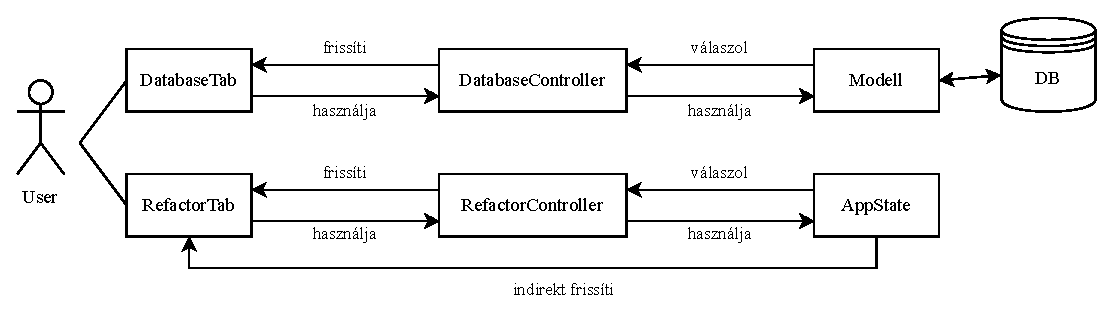
\includegraphics[width=0.9\textwidth]{images/figs/MVC.eps}
	\caption{\label{fig:MVC}Egy esemény kezelése az alkalmazás architektúrájában}
\end{figure}

Az alkalmazásban csak a \emph{RefactorController} végez indirekt frissítést a
\ref{subsec:appstate}. alcím alatt részletezett \emph{Observable} tervezési minta
segítségével. 

\section{Modulok}
\label{sec:modules}

A csomagok a \emph{tests} csomagon kívül nem tartalmaznak futtatásra szánt fájlokat.
A belépési pontok és segédfüggvények a \ref{tab:modules}. táblázatban
látható modulokba vannak szervezve.

\begin{table}[H]
	\centering
	\begin{tabular}{ | m{0.25\textwidth} | m{0.65\textwidth} | }
		\hline
		\textbf{Modul} & \textbf{Rövid leírás} \\
		\hline \hline
		\emph{launch} & GUI alkalmazás belépési pontjának modulja \\
		\hline
		\emph{persistor} & CLI program modulja \\
		\hline
		\emph{tools} & modul eszközök alkalmazására (pl. linterek) \\
		\hline
		\emph{utils} & utility függvények modulja (pl. fájlok olvasásához)  \\
		\hline
	\end{tabular}
	\caption{A szoftver fő moduljai}
	\label{tab:modules}
\end{table}

A \emph{lanuch} modul \emph{main} függvénye a GUI alkalmazást példányosítja.
A \emph{persistor} modulban az adathalmazt generáló CLI program implementációja található.

A \emph{tools} és \emph{utils} modulok segédfüggvények definícióit tartalmazzák,
a \emph{ruff} lintert alkalmazó függvények például a \emph{tools} modulban,
az IO műveleteket végző függvények pedig a \emph{utils} modulban találhatóak.

\pagebreak

\section{Tesztelés}

Az átalakító szabályok tesztelését \emph{unittest} modulban írt egységtesztekkel végzem.
Az egységtesztek mellett az átalakítások tesztelésére a \emph{QuixBugs}
benchmarkot \cite{QuixBugs} is felhasználtam.
A \emph{QuixBugs}-os tesztek működéséről a \ref{sec:QuixBugs}. szekcióban olvashatunk.

\subsection{Egységtesztek}

Az egységtesztek forráskódját a \emph{tests.unit} csomag \emph{\_\_main\_\_}
moduljában találjuk. A tesztek futtatásához a modul \emph{main} függvényét kell meghívni.

A teszteseteket a \emph{unittest.TestCase}-ből származó osztályok reprezentálják.
Egy tesztesethez több teszt is tartozik, ezek a teszteset osztályának metódusai.
A teszteseteket és a hozzájuk tartozó teszteket a \ref{tab:unit_tests}. táblázatban láthatjuk.

Egy teszt egy előre megadott forráskódokon alkalmaz egy szabályt.
Ha a szabály alkalmazása után a kapott eredmény egyezik az elvárt eredménnyel
(lásd \ref{tab:unit_tests}. táblázat \emph{Eredmény} oszlopa), akkor a teszt sikeres.

\lstset{
	caption={},
	numbers=none,
}

\begin{center}
	\begin{longtable}{ | p{0.25\textwidth} | p{0.45\textwidth} | p{0.2\textwidth} | }
		\hline
		\multicolumn{3}{ |c| }{\textbf{Egységtesztek}}
		\\ \hline
		
		\textbf{Teszt} & \textbf{Rövid leírás} & \textbf{Eredmény}
		\\ \hline \hline
		\endfirsthead % első oldal fejléce
		
		\hline
		\textbf{Teszt} & \textbf{Rövid leírás} & \textbf{Eredmény}
		\\ \hline \hline
		\endhead % többi oldal fejléce
		
		\hline
		\endfoot % többi oldal lábléce
		
		\endlastfoot % utolsó oldal lábléce
		
		\multicolumn{3}{ |l| }{\textbf{\texttt{TestForRules}} teszteset:}
		\\ \hline
		
		\texttt{\lstinline{test_for_to_dict}}
		&
		$ForToDictComprehension$ szabály
		
		alkalmazása átalakítható kódokon
		&
		a kódok helyesen átalakulnak
		\\
		\hline
		
		\texttt{\lstinline{test_for_to_list}}
		&
		$ForToListComprehension$ szabály
		
		alkalmazása átalakítható kódokon
		&
		a kódok helyesen átalakulnak
		\\
		\hline

		\texttt{\lstinline{test_for_to_set}}
		&
		$ForToSetComprehension$ szabály
		
		alkalmazása átalakítható kódokon
		&
		a kódok helyesen átalakulnak
		\\
		\hline

		\texttt{\lstinline{test_for_to_sum}}
		&
		$ForToSum$ szabály

		alkalmazása átalakítható kódokon
		&
		a kódok helyesen átalakulnak
		\\
		\hline

		\texttt{\lstinline{test_name_count}}
		&
		$For$ node-ban található

		$Name$ node-ok számára

		vonatkozó feltétel tesztelése
		&
		a feltételnek

		megfelelő kódok
		átalakulnak
		\\
		\hline

		\texttt{\lstinline{test_control_flow}}
		&
		$Assign$ node és $For$ node közötti

		node-okra vonatkozó feltétel

		tesztelése
		&
		a feltételnek

		megfelelő kódok
		átalakulnak
		\\
		\hline

		\multicolumn{3}{ |l| }{\textbf{\texttt{TestSimpleRules}} teszteset:}
		\\ \hline

		\texttt{\lstinline{test_invert_if}}
		&
		$InvertIf$ szabály

		alkalmazása átalakítható kódokon
		&
		a kódok helyesen átalakulnak
		\\
		\hline

		\texttt{\lstinline{test_single_if}}
		&
		$SingleIf$ szabállyal felismert

		$If$ node else ágra vonatkozó

		feltétel tesztelése
		&
		a feltételnek
		
		megfelelő kódok
		átalakulnak
		\\
		\hline

		\texttt{\lstinline{test_de_morgan}}
		&
		$DeMorgan$ szabály

		alkalmazása átalakítható kódokon
		&
		a kódok helyesen átalakulnak
		\\ \hline

		\texttt{\lstinline{test_better_neg}}
		&
		$BetterNegation$ szabály

		alkalmazása átalakítható kódokon
		&
		a kódok helyesen átalakulnak
		\\ \hline

		\texttt{\lstinline{test_double_neg}}
		&
		$DoubleNegation$ szabállyal felismert
		
		$UnaryOp$ operandusaira vonatkozó

		feltétel tesztelése
		&
		a feltételnek

		megfelelő kódok
		átalakulnak
		\\ \hline

		\texttt{\lstinline{test_tuple_assign_1}}
		&
		$TupleAssign$ szabály

		alkalmazása egy átalakítható kódon
		&
		a kód helyesen átalakul
		\\ \hline

		\texttt{\lstinline{test_tuple_assign_2}}
		&
		$TupleAssign$ szabály alkalmazása

		nem megfelelő értékadást tartamazó kódon
		&
		nincs átalakítás
		\\ \hline

		\texttt{\lstinline{test_mult_assign_1}}
		&
		$MultipleAssign$ szabály

		alkalmazása egy átalakítható kódon
		&
		a kód helyesen átalakul
		\\ \hline

		\texttt{\lstinline{test_mult_assign_2}}
		&
		$MultipleAssign$ szabály alkalmazása

		nem megfelelő értékadást tartamazó kódon
		&
		nincs átalakítás
		\\ \hline \hline

		\multicolumn{3}{ |l| }{\textbf{\texttt{TestProbabilityRules}} teszteset:}
		\\ \hline

		\texttt{\lstinline{test_commut_mult_1}}
		&
		$CommutativeMult$ szabály
		
		alkalmazása egy átalakítható kódon
		&
		a kód helyesen átalakul
		\\
		\hline

		\texttt{\lstinline{test_commut_mult_2}}
		&
		$CommutativeMult$ szabály
		
		alkalmazása egy átalakítható kódon
		&
		a kód helyesen átalakul
		\\
		\hline

		\texttt{\lstinline{test_commut_mult_3}}
		&
		$CommutativeMult$ szabály

		alkalmazása két nem $Constant$ node közti szorzásra
		&
		nincs átalakítás
		\\
		\hline

		\texttt{\lstinline{test_insert_continue}}
		&
		$InsertContinue$ szabály
	
		alkalmazása egy átalakítható kódon
		&
		a kód helyesen átalakul
		\\
		\hline

		\texttt{\lstinline{test_insert_pass}}
		&
		$InsertPass$ szabály
		
		alkalmazása egy átalakítható kódon
		&
		a kód helyesen átalakul
		\\ \hline

		\multicolumn{3}{ |l| }{\textbf{\texttt{TestNonEquivalentRules}} teszteset:}
		\\ \hline

		\texttt{\lstinline{test_negate_if}}
		&
		$NeqvNegateIf$ szabály
		
		alkalmazása egy átalakítható kódon
		&
		a kód helyesen átalakul
		\\
		\hline

		\texttt{\lstinline{test_invert_if}}
		&
		$NeqvInvertIf$ szabály
		
		alkalmazása egy átalakítható kódon
		&
		a kód helyesen átalakul
		\\
		\hline

		\texttt{\lstinline{test_swap_and_or}}
		&
		$NeqvSwapAndOr$ szabály
		
		alkalmazása egy átalakítható kódon
		&
		a kód helyesen átalakul
		\\
		\hline

		\texttt{\lstinline{test_swap_add_sub}}
		&
		$NeqvSwapAddSub$ szabály
		
		alkalmazása egy átalakítható kódon
		&
		a kód helyesen átalakul
		\\
		\hline

		\texttt{\lstinline{test_insert_return}}
		&
		$NeqvInsertReturn$ szabály
		
		alkalmazása egy átalakítható kódon
		&
		a kód helyesen átalakul
		\\
		\hline

		\caption{Egységtesztek táblázata}
		\label{tab:unit_tests}
	\end{longtable}
\end{center}

\pagebreak

\subsection{Tesztelés a \emph{QuixBugs} segítségével\label{sec:QuixBugs}}


A \emph{QuixBugs} benchmark eredeti célja a forráskód-javításra képes eszközök tesztelése,
de a benchmarkot használhatjuk forráskódokon végzett átalakítások tesztelésére is.

A \emph{QuixBugs} benchmark 40 közismert algoritmus Java és Python implementációját tartalmazza.
Minden algoritmushoz található egy helyes és egy helytelen (bugos) implementáció.
Az algoritmusokhoz előre megírt tesztek is tartoznak.

A benchmark segítségével egyszerre több átalakító szabályt tesztelek.
Ehhez az algoritmusok forráskódjait előbb átalakítom, majd futtatom a \emph{QuixBugs}
teszteseteit az átalakított kódokon.

Az ekvivalens szabályok akkor helyesek, ha nem ronthatnak el egy kódot sem,
vagyis ha az átalakított kódokon futtatott összes teszt eredménye sikeres.
Azt is tesztelem, hogy egy nem ekvivalens szabály képes-e elrontani egy kódot,
vagyis úgy átalakítani a kódot, hogy a hozzá tartozó tesztek elbukjanak.

A benchmarkot használó teszteket a \emph{tests.quix} csomag \emph{\_\_main\_\_} moduljában található
\emph{main} függvénnyel futtathatjuk.
A tesztek futtatásához szükségünk van a \emph{QuixBugs} repóra, a \emph{main} függvényt
a repó elérési útvonalával kell meghívni.

A teszteteket a \emph{test\_transformations} függvény végzi,
ez a függvénnyel teszteli az általam implementált összes ekvivalens és nem ekvivalens szabályt.
Az alkalmazott szabályok ekvivalenciáját az \emph{equivalent} paraméterrel lehet megadni.

A \emph{test\_transformations} által végzett teszteknek két fázisa van.
A függvény először a cache-eli az összes helyes megoldást tartalmazó forrráskódot,
ezután átalakítja a forráskódokat és futtatja a \emph{QuixBugs} tesztjeit.
Ha a tesztek lefutottak a cache-elt kódok felülírják az átalakított kódokat,
így újraindíthatjuk a tesztet.

A \emph{QuixBugs}-os teszteket többször is futtattam,
a tesztek eredményeit a \ref{tab:quix_tests}. táblázatban láthatjuk.
A táblázat egy sora egy teszt eredményeit tartalmazza.

Az első két oszlopban a sikeres tesztek és végzett tesztek számának százalékos aránya (\emph{Pass\%})
szerepel ekvivalens és nem ekvivalens szabályok alkalmazása után.
Egy tesztet akkor tekintek sikeresnek, ha ekvivalens szabályok esetén a \emph{Pass\%} 100,
vagyis ha az ekvivalens szabályok nem rontanak el egy kódot sem.

\begin{table}[H]
	\centering
	\begin{tabular}{ | m{0.45\textwidth} | m{0.45\textwidth} | }
		\hline
		\textbf{Pass\%}
		
		\textbf{ekvivalens szabályoknál}
		&
		\textbf{Pass\%}
		
		\textbf{nem ekvivalens szabályoknál}
		\\
		\hline \hline
		276 / 276 = 100\% & 31 / 276 $\approx$ 11\% \\
		\hline
		276 / 276 = 100\% & 23 / 276 $\approx$ 8\% \\
		\hline
		276 / 276 = 100\% & 30 / 276 $\approx$ 10\% \\
		\hline
		276 / 276 = 100\% & 14 / 276 $\approx$ 5\% \\
		\hline
		276 / 276 = 100\% & 26 / 276 $\approx$ 9\% \\
		\hline
	\end{tabular}
	\caption{\emph{QuixBugs} benchmarkot használó tesztek eredményei}
	\label{tab:quix_tests}
\end{table}

A \ref{tab:quix_tests}. táblázatban látható, hogy a nem ekvivalens szabályok alkalmazása után
a kódok nagy része nem megy át a teszteseteken.
A nem ekvivalens szabályok esetében az eredmények azért különböznek,
mert a szabályok alkalmazásának alap valószínűsége kisebb mint 1,
ezért az összes nem ekvivalens szabályt alkalmazó függvény nem determinisztikus.

\pagebreak
